\documentclass[aspectratio=169,10pt]{beamer}

% ------------------------------------------------------------
% Modern Light Blue + Navy Beamer Colloquium Presentation
% ------------------------------------------------------------
\usetheme{Madrid}
\usefonttheme{professionalfonts}

\usepackage[T1]{fontenc}
\usepackage[utf8]{inputenc}
\usepackage{lmodern}
\usepackage{graphicx}
\usepackage{booktabs}
\usepackage{array}
\usepackage{tabularx}
\usepackage{multirow}
\usepackage{ragged2e}
\usepackage{tikz}
\usetikzlibrary{positioning,arrows.meta,shapes.geometric,calc,fit,backgrounds}
\usepackage{hyperref}
\usepackage{xcolor}
\usepackage{amsmath}
\usepackage{pifont}
\usepackage{makecell}
\usepackage{adjustbox}

% ---------------------- Colors -----------------------------
\definecolor{Navy}{HTML}{0B1F4D}
\definecolor{NavyTwo}{HTML}{123C69}
\definecolor{Cyan}{HTML}{00AEEF}
\definecolor{CyanSoft}{HTML}{D7ECFF}
\definecolor{Teal}{HTML}{008EA6}
\definecolor{Gold}{HTML}{D6A11B}
\definecolor{Slate}{HTML}{1A1A1A}
\definecolor{Muted}{HTML}{536B84}
\definecolor{Card}{HTML}{EAF3FF}
\definecolor{DarkCard}{HTML}{FFFFFF}
\definecolor{Alert}{HTML}{C0392B}
\definecolor{Green}{HTML}{218C5A}
\definecolor{LightBlueBG}{HTML}{F4F8FF}

% ---------------------- Beamer Theme -----------------------
\setbeamercolor{normal text}{fg=Slate,bg=LightBlueBG}
\setbeamercolor{background canvas}{bg=LightBlueBG}
\setbeamercolor{frametitle}{fg=white,bg=Navy}
\setbeamercolor{title}{fg=Navy}
\setbeamercolor{subtitle}{fg=NavyTwo}
\setbeamercolor{author}{fg=Slate}
\setbeamercolor{institute}{fg=Slate}
\setbeamercolor{date}{fg=Gold}
\setbeamercolor{structure}{fg=NavyTwo}
\setbeamercolor{itemize item}{fg=Cyan}
\setbeamercolor{itemize subitem}{fg=Teal}
\setbeamercolor{enumerate item}{fg=Cyan}
\setbeamercolor{block title}{fg=white,bg=NavyTwo}
\setbeamercolor{block body}{fg=Slate,bg=Card}
\setbeamercolor{block title alerted}{fg=white,bg=Alert}
\setbeamercolor{block body alerted}{fg=Slate,bg=CyanSoft}
\setbeamercolor{block title example}{fg=white,bg=Cyan}
\setbeamercolor{block body example}{fg=Slate,bg=DarkCard}
\setbeamercolor{caption name}{fg=NavyTwo}

\setbeamertemplate{navigation symbols}{}
\setbeamertemplate{caption}[numbered]
\setbeamertemplate{bibliography item}{\insertbiblabel}
\setbeamerfont{caption}{size=\scriptsize}
\setbeamerfont{bibliography item}{size=\scriptsize}
\setbeamerfont{bibliography entry author}{size=\scriptsize}
\setbeamerfont{bibliography entry title}{size=\scriptsize}
\setbeamerfont{bibliography entry location}{size=\scriptsize}
\setbeamerfont{bibliography entry note}{size=\scriptsize}

\hypersetup{
  colorlinks=true,
  linkcolor=NavyTwo,
  urlcolor=Teal,
  citecolor=Gold
}

% ---------------------- Footline ---------------------------
\setbeamertemplate{footline}{%
  \leavevmode%
  \hbox{%
    \begin{beamercolorbox}[wd=.34\paperwidth,ht=2.8ex,dp=1.2ex,leftskip=1em]{author in head/foot}%
      \usebeamerfont{author in head/foot}\color{white}Tanneeru Vidath \;|\; ABV-IIITM
    \end{beamercolorbox}%
    \begin{beamercolorbox}[wd=.44\paperwidth,ht=2.8ex,dp=1.2ex,center]{title in head/foot}%
      \usebeamerfont{title in head/foot}\color{white}Optimized Task Offloading in Healthcare IoT-Fog Systems
    \end{beamercolorbox}%
    \begin{beamercolorbox}[wd=.22\paperwidth,ht=2.8ex,dp=1.2ex,right,rightskip=1em]{date in head/foot}%
      \usebeamerfont{date in head/foot}\color{white}\insertframenumber{} / \inserttotalframenumber
    \end{beamercolorbox}%
  }%
  \vskip0pt%
}

% ---------------------- Utility Commands -------------------
\newcommand{\cmark}{\textcolor{Green}{\ding{51}}}
\newcommand{\xmark}{\textcolor{Alert}{\ding{55}}}

\newcolumntype{Y}{>{\RaggedRight\arraybackslash}X}
\newcolumntype{C}[1]{>{\centering\arraybackslash}p{#1}}
\newcolumntype{L}[1]{>{\RaggedRight\arraybackslash}p{#1}}

\newcommand{\bgdecor}{%
\begin{tikzpicture}[remember picture,overlay]
  \fill[Cyan,opacity=.12] ($(current page.north east)+(-3.6,-.4)$) circle (2.8cm);
  \fill[NavyTwo,opacity=.06] ($(current page.south west)+(2.2,1.0)$) circle (2.3cm);
  \draw[NavyTwo,opacity=.30,line width=0.8pt]
    ($(current page.north west)+(0.2,-0.85)$) --
    ($(current page.north east)+(-0.2,-0.85)$);
\end{tikzpicture}}

\newcommand{\ImageOrPlaceholder}[4][0.65\textheight]{%
\IfFileExists{#2}{%
  \includegraphics[width=#3,height=#1,keepaspectratio]{#2}%
}{%
\begin{tikzpicture}
\node[
draw=Cyan,
line width=0.7pt,
rounded corners=8pt,
fill=Card,
minimum width=#3,
minimum height=#1,
align=center
] {\textcolor{Cyan}{\Large #4}\\[3pt]
\textcolor{Muted}{\scriptsize \texttt{\detokenize{#2}}}};
\end{tikzpicture}}}

% ---------------------- Title Metadata ---------------------
\title[Optimized Task Offloading]{Optimized Task Offloading for Healthcare IoT-Fog Systems}
\subtitle{Severity-Aware 2-Type Multi-Stage Deferred Acceptance Framework}
\author[Tanneeru Vidath]{\textbf{Tanneeru Vidath}\\Roll No.: 2023BCS-068}
\institute[ABV-IIITM Gwalior]{Department of Computer Science and Engineering\\Atal Bihari Vajpayee Indian Institute of Information Technology and Management, Gwalior}
\date{Summer Colloquium \; | \; August 2026}

\begin{document}

% ============================================================
% SLIDE 1: Title Slide
% ============================================================
\begin{frame}[plain,label=title]{}
\bgdecor
\centering

{\LARGE\bfseries\textcolor{Navy}{Optimized Task Offloading for Healthcare IoT-Fog Systems}}\\[0.06cm]

{\normalsize\textcolor{Gold}{Summer Colloquium Presentation \; | \; August 2026}}\\[0.18cm]

{\Large\textbf{Tanneeru Vidath}}\\[-1pt]
{\small Roll No: 2023BCS-068}\\[0.10cm]

\IfFileExists{FrontPages/ABV_IIITM_Logo.jpeg}{%

\includegraphics[width=1.35cm]{FrontPages/ABV_IIITM_Logo.jpeg}%
}{%

\begin{tikzpicture}
\node[draw=Cyan, fill=Card, rounded corners=6pt, inner sep=4pt]
{\textcolor{Navy}{ABV-IIITM}};
\end{tikzpicture}%
}\\[0.10cm]

{\small Department of Computer Science and Engineering\\ABV-IIITM Gwalior, M.P. -- 474015}\\[0.14cm]

{\large\textbf{Supervisor:}}\\[-1pt]
{\small\textbf{Dr. Chittaranjan Swain}}
\end{frame}

% ============================================================
% SLIDE 2: Presentation Outline
% ============================================================
\begin{frame}[label=outline]{Presentation Outline}
\bgdecor

\vspace{0.05cm}
\begin{block}{Project Focus}
\centering
\textbf{Enhancing Task Offloading Fairness and Eliminating Life-Critical Task Outages in Healthcare IoT-Fog Networks}
\end{block}

\vspace{0.15cm}

\begin{columns}[T,onlytextwidth]
\column{0.32\textwidth}
\begin{block}{Background \& Context}
\small
\begin{enumerate}
  \item Introduction \& Motivation
  \item Literature Review
  \item Problem Statement
\end{enumerate}
\end{block}

\column{0.32\textwidth}
\begin{block}{Proposed Solution}
\small
\begin{enumerate}
  \setcounter{enumi}{3}
  \item Solution: Overview
  \item Delay, Energy \& Prefs
  \item Urgency \& Precedence
  \item 3-Tier Quota Framework
  \item Adapted MSDA Algorithm
\end{enumerate}
\end{block}

\column{0.33\textwidth}
\begin{block}{Implementation \& Results}
\small
\begin{enumerate}
  \setcounter{enumi}{8}
  \item Tech Stack \& Setup
  \item Results: Outage
  \item Results: Delay
  \item Limitations \& Future
\end{enumerate}
\end{block}
\end{columns}
\end{frame}

% ============================================================
% SLIDE 3: Introduction & Motivation
% ============================================================
\begin{frame}[label=intro]{Introduction \& Motivation}
\bgdecor

\begin{columns}[T,onlytextwidth]
\column{0.48\textwidth}
\begin{block}{Healthcare IoT \& Fog Computing}
\small
\begin{itemize}
  \item \textbf{IoT in Healthcare}: Modern hospitals rely on interconnected medical devices (e.g., robotic surgeries, ECG monitors) generating massive time-critical data.
  \item \textbf{Why Fog Computing?}: Cloud latency is too high. Fog nodes (local edge servers) process data closer to devices, delivering \textbf{low-latency} response for life-critical operations.
\end{itemize}
\end{block}

\column{0.48\textwidth}
\begin{exampleblock}{The Task Offloading Challenge}
\small
\begin{itemize}
  \item Devices must ``offload'' heavy processing tasks to fog nodes.
  \item \textbf{Bottleneck}: Fog nodes have limited CPU and VRU capacity. Under congestion, tasks compete for resources.
  \item \textbf{Goal}: An intelligent system to \textbf{match} tasks to fog nodes without violating strict deadlines.
\end{itemize}
\end{exampleblock}
\end{columns}
\end{frame}

% ============================================================
% SLIDE 4: Literature Review
% ============================================================
\begin{frame}[label=lit_review]{Literature Review}
\bgdecor

\scriptsize
\renewcommand{\arraystretch}{1.28}
\begin{adjustbox}{max width=\textwidth, max height=.80\textheight}
\begin{tabular}{L{2.5cm} L{3.5cm} L{4.0cm} L{3.6cm}}
\toprule
\textbf{Author / Paper} & \textbf{Problem Identified} & \textbf{Solution Approach} & \textbf{Constraints Considered}\\
\midrule

Gale \& Shapley \newline (1962) \cite{gale1962}
& Stable matching in two-sided markets without quotas.
& Introduced the \textbf{Deferred Acceptance (DA)} algorithm.
& Strict preferences, stability, capacity limits (no min quotas).\\
\midrule

Kamada \& Kojima \newline (2015) \cite{kamada2015}
& Standard DA fails to guarantee fairness when minimum quotas are required.
& Extended DA to \textbf{Multi-Stage DA (MSDA)} enforcing quotas iteratively.
& Regional minimum quotas, overall maximum capacities.\\
\midrule

Oomori \& Manabe \newline (2026) \cite{oomori2026}
& Assigning two distinct agent types fairly with overlapping quota requirements.
& Proposed \textbf{2-Type MSDA} to handle disjoint minimum and maximum limits.
& Separate agent types, simultaneous minimum and maximum quotas.\\
\midrule



Swain et al. (2024) \newline \textit{M-DAFTO} \cite{swain2024}
& Fair and scalable assignment of deadline-sensitive IoT tasks.
& \textbf{MSDA} combined with AHP-TOPSIS urgency and precedence lists.
& Deadlines, single min/max quotas, feasible options.\\
\bottomrule
\end{tabular}
\end{adjustbox}
\end{frame}

% ============================================================
% SLIDE 5: Problem Statement
% ============================================================
\begin{frame}[label=problem]{Problem Statement}
\bgdecor

\begin{columns}[T,onlytextwidth]
\column{0.48\textwidth}
\begin{alertblock}{The Core Challenge: Task Starvation}
\small
In smart hospitals, tasks are highly heterogeneous. Critical robotic surgeries (millisecond-latency) run alongside routine telemetry. Under high load, unmanaged competition causes \textbf{outages}---life-critical operations fail to meet their deadlines.
\end{alertblock}

\column{0.48\textwidth}
\begin{alertblock}{Identified Research Gaps (M-DAFTO)}
\small
M-DAFTO is state-of-the-art for general IoT, but has critical gaps for healthcare:
\begin{itemize}
  \item \textbf{Single-Pool Competition}: Treats surgeries and checkups equally $\Rightarrow$ starvation.
  \item \textbf{No Energy Awareness}: Urgency uses only delay \& preference count (2 criteria).
  \item \textbf{Single-Tier Quotas}: Only global min/max ($p_j, q_j$) --- cannot enforce separate guarantees for Major vs Minor tasks.
\end{itemize}
\end{alertblock}
\end{columns}
\end{frame}

% ============================================================
% SLIDE 6: Proposed Solution: Overview
% ============================================================
\begin{frame}[label=solution_overview]{Proposed Solution: Overview}
\bgdecor

\vspace{-0.1cm}
\begin{center}
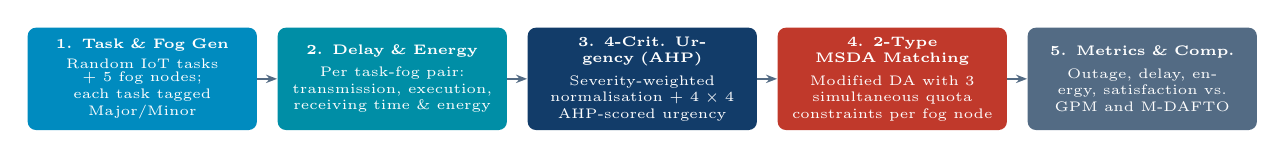
\begin{tikzpicture}[
  node distance=0.25cm,
  box/.style={
    align=center, 
    font=\fontsize{5}{6}\selectfont\color{white}, 
    rounded corners=3pt, 
    inner sep=3pt, 
    minimum height=1.3cm,
    minimum width=2.85cm,
    text width=2.7cm
  },
  arr/.style={-{Stealth[length=4pt]}, thick, draw=Muted}
]

\node[box, fill=Cyan!80!black] (n1) {\textbf{1. Task \& Fog Gen}\\[2pt] \fontsize{4}{5}\selectfont Random IoT tasks + 5 fog nodes;\\each task tagged Major/Minor};
\node[box, fill=Teal, right=of n1] (n2) {\textbf{2. Delay \& Energy}\\[2pt] \fontsize{4}{5}\selectfont Per task-fog pair: transmission, execution, receiving time \& energy};
\node[box, fill=NavyTwo, right=of n2] (n3) {\textbf{3. 4-Crit. Urgency (AHP)}\\[2pt] \fontsize{4}{5}\selectfont Severity-weighted normalisation + $4\times4$ AHP-scored urgency};
\node[box, fill=Alert, right=of n3] (n4) {\textbf{4. 2-Type MSDA Matching}\\[2pt] \fontsize{4}{5}\selectfont Modified DA with 3 simultaneous quota constraints per fog node};
\node[box, fill=Muted, right=of n4] (n5) {\textbf{5. Metrics \& Comp.}\\[2pt] \fontsize{4}{5}\selectfont Outage, delay, energy, satisfaction vs. GPM and M-DAFTO};

\draw[arr] (n1) -- (n2);
\draw[arr] (n2) -- (n3);
\draw[arr] (n3) -- (n4);
\draw[arr] (n4) -- (n5);
\end{tikzpicture}
\end{center}
\vspace{-0.1cm}

\begin{columns}[T,onlytextwidth]
\column{0.48\textwidth}
\begin{block}{IoT Task Model ($T_i$, $i=1\ldots M$)}
\small
\begin{itemize}
  \item $\text{cpuDemanded}_i \in [210, 480]$ Mcycles
  \item $\text{inputSize}_i \in [300, 600]$ KB
  \item $\text{outputSize}_i \in [10, 20]$ KB
  \item $\text{deadline}_i \in [15, 22]$ seconds
  \item $\text{severity}_i$: \textbf{Major} or \textbf{Minor}
  \item $\text{phase}_i$: Pre-Surgery / Post-Surgery
\end{itemize}
\end{block}

\column{0.48\textwidth}
\begin{block}{Fog Node Model ($F_j$, $j=1\ldots N$)}
\small
\begin{itemize}
  \item $\text{totalCpuGHz}_j \in [6.0, 10.0]$ GHz
  \item $\text{numberOfVRUs}_j \in [200, 500]$
  \item $\text{vruCapacity}_j = \frac{\text{totalCpu} \times 1000}{\text{VRUs}}$ Mcycles/s
  \item $P_{tx}=0.5$W, $P_{exec}=1.0$W, $P_{rx}=0.5$W
\end{itemize}
A VRU is a logical unit of compute capacity. Max quota of a fog node = its number of VRUs.
\end{block}
\end{columns}

% You can replace this placeholder with your actual flowchart image later:
% \vspace{0.1cm}\centering
% \ImageOrPlaceholder[2.2cm]{Images/proposed_solution_flowchart.png}{0.7\linewidth}{Flowchart}
\end{frame}

% ============================================================
% SLIDE 7: Offloading Delay, Energy & Task Preferences
% ============================================================
\begin{frame}[label=task_prefs]{Offloading Delay, Energy \& Task Preferences}
\bgdecor

\begin{block}{Offloading Delay \& Energy Formulations}
\small
For task $T_i$ offloaded to fog node $F_j$:
\begin{columns}[T,onlytextwidth]
\column{0.48\textwidth}
\begin{itemize}
  \item \textbf{Transmission Time}: $t_{ij}^{tx} = \dfrac{\text{inputSize}_i}{\text{UPLINK\_RATE}}$
  \item \textbf{Execution Time}: $t_{ij}^{exec} = \dfrac{\text{cpuDemanded}_i}{\text{vruCapacity}_j}$
  \item \textbf{Reception Time}: $t_{ij}^{rx} = \dfrac{\text{outputSize}_i}{\text{DOWNLINK\_RATE}}$
\end{itemize}
\column{0.48\textwidth}
\begin{itemize}
  \item \textbf{Total Delay}: $\text{delay}_{ij} = t_{ij}^{tx} + t_{ij}^{exec} + t_{ij}^{rx}$
  \item Must satisfy: $\text{delay}_{ij} \le \text{deadline}_i$
  \item \textbf{Energy}: $E_{ij} = P_{tx} t_{ij}^{tx} + P_{exec} t_{ij}^{exec} + P_{rx} t_{ij}^{rx}$
  \item Uplink/Downlink: 2500 KB/s (20 MHz BW)
\end{itemize}
\end{columns}
\end{block}

\begin{exampleblock}{Normalisation \& Task Preference Lists}
\small
Values are severity-weighted min-max normalised: $nd_{ij}$, $ne_{ij}$ (weight = 1.0 for Major, 0.5 for Minor).
Every task ranks fog nodes by ascending \textbf{normSum}:
$\text{Cost}(T_i, F_j) = nd_{ij} + ne_{ij}$
\quad$\Rightarrow$ Tasks always propose to lowest-cost fog nodes first.
\end{exampleblock}
\end{frame}

% ============================================================
% SLIDE 8: Urgency Model (AHP) & Fog Preferences & Precedence
% ============================================================
\begin{frame}[label=fog_prefs]{Urgency Model (AHP), Fog Preferences \& Precedence}
\bgdecor

\begin{columns}[T,onlytextwidth]
\column{0.50\textwidth}
\begin{block}{Fog Preferences: 4-Criteria Urgency}
\small
Each fog node $F_j$ ranks tasks by urgency:
\[ U(T_i, F_j) = w_1 \frac{1}{\Delta d} + w_2 \frac{1}{\text{pref}(T_i)} + w_3 \frac{1}{ne_{ij}} + w_4 \gamma(T_i) \]
where $\Delta d = \text{deadline}_i - \text{delay}_{ij}$, \; $\text{pref}(T_i) = $ feasible fog count, and $\gamma(T_i) = 1 + c_i \times 0.5$ (so $\gamma=1.5$ for Major, $1.0$ for Minor).

\vspace{0.1cm}
Fog nodes generate \textbf{3 ranked lists}: all tasks, Major-only, Minor-only.
\end{block}

\column{0.48\textwidth}
\begin{block}{AHP Weight Generation ($4\times 4$)}
\small
\begin{enumerate}
  \item \textbf{PMC}: Build $4\times 4$ pairwise matrix $P$ using Saaty scale ratios.
  \item \textbf{CWD}: Column-normalise $P$ and row-average $\to W = [w_1 \ldots w_4]^T$.
  \item \textbf{CC}: Compute $\lambda_{max}$, then $CR = \frac{(\lambda_{max}-n)/(n-1)}{RI}$ with $RI=0.90$. Accept only if $CR \le 0.10$.
\end{enumerate}
\end{block}

\begin{block}{Precedence Lists}
\small
Tasks sorted strictly by deadline $\to$ tightest deadlines propose first. Separate lists for Major \& Minor tasks.
\end{block}
\end{columns}
\end{frame}

% ============================================================
% SLIDE 9: 3-Tier Quota Framework
% ============================================================
\begin{frame}[label=quota]{3-Tier Quota Framework}
\bgdecor

\begin{columns}[T,onlytextwidth]
\column{0.50\textwidth}
\begin{block}{Minimum Quota Determination (MQD)}
\scriptsize
Base minimums are proportional to VRU capacity relative to the most efficient node ($\lambda_{\max}$):
\vspace{2pt}
\begin{center}
$p_c = \min\left( \left\lfloor \frac{\text{vruCapacity}_c}{\lambda_{\max}} \times l_{\max} \right\rfloor, \, q_c \right)$
\end{center}
\vspace{2pt}
where $l_{\max} = \min(h_{\max}, \lfloor |T|/|F| \rfloor)$, and $h_{\max}$ is max VRUs.
\end{block}

\begin{block}{3-Tier Quota Variables per Fog Node $c$}
\scriptsize
\textbf{Minimums (Floors):}\\
$p_c$: All tasks (fairness) \quad $pr_c$: Major tasks (anti-starvation)\\[4pt]
\textbf{Maximums (Ceilings):}\\
\textbf{All tasks}: $q_c$ \quad \textbf{Major}: $qr_c$ \quad \textbf{Minor}: $q_c - pr_c$
\end{block}

\column{0.48\textwidth}
\centering
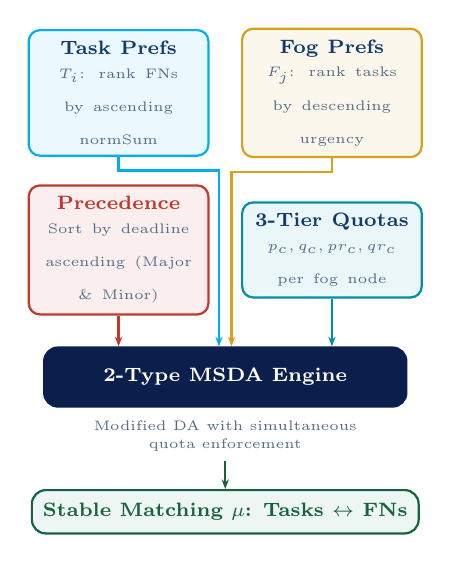
\begin{tikzpicture}[
  node distance=0.2cm,
  every node/.style={align=center},
  inbox/.style={rounded corners=4pt, minimum width=2.1cm, text width=2cm, inner sep=4pt, draw, thick},
  enginebox/.style={rounded corners=5pt, minimum width=4.6cm, minimum height=0.75cm, draw=Navy, thick, fill=Navy, text=white, font=\scriptsize\bfseries, inner sep=5pt},
  outbox/.style={rounded corners=5pt, minimum width=4.2cm, minimum height=0.55cm, draw=Green!70!black, thick, fill=Green!8, font=\scriptsize\bfseries, inner sep=4pt},
  arr/.style={-{Stealth[length=3.5pt]}, thick, NavyTwo}
]
% Row 1
\node[inbox, draw=Cyan, fill=Cyan!8] (tpref) {
  {\scriptsize\bfseries\textcolor{NavyTwo}{Task Prefs}}\\[2pt]
  {\fontsize{5}{6.5}\selectfont\textcolor{Muted}{$T_i$: rank FNs\\by ascending normSum}}
};
\node[inbox, draw=Gold, fill=Gold!8, right=0.4cm of tpref] (fpref) {
  {\scriptsize\bfseries\textcolor{NavyTwo}{Fog Prefs}}\\[2pt]
  {\fontsize{5}{6.5}\selectfont\textcolor{Muted}{$F_j$: rank tasks\\by descending urgency}}
};

% Row 2
\node[inbox, draw=Alert, fill=Alert!8, below=0.35cm of tpref] (prec) {
  {\scriptsize\bfseries\textcolor{Alert}{Precedence}}\\[2pt]
  {\fontsize{5}{6.5}\selectfont\textcolor{Muted}{Sort by deadline\\ascending (Major \& Minor)}}
};
\node[inbox, draw=Teal, fill=Teal!8, right=0.4cm of prec] (quota) {
  {\scriptsize\bfseries\textcolor{NavyTwo}{3-Tier Quotas}}\\[2pt]
  {\fontsize{5}{6.5}\selectfont\textcolor{Muted}{$p_c, q_c, pr_c, qr_c$\\per fog node}}
};

% Engine
\node[enginebox, below=0.5cm of $(prec.south)!0.5!(quota.south)$] (engine) {2-Type MSDA Engine};
\node[below=0.05cm of engine, font=\fontsize{5}{6.5}\selectfont, text=Muted] (esub) {Modified DA with simultaneous\\quota enforcement};

% Output
\node[outbox, below=0.35cm of esub, text=Green!70!black] (out) {Stable Matching $\mu$: Tasks $\leftrightarrow$ FNs};

% Arrows
\draw[arr, Cyan] (tpref.south) -- ++(0,-0.175) -| ([xshift=-0.08cm]engine.north);
\draw[arr, Gold] (fpref.south) -- ++(0,-0.175) -| ([xshift=0.08cm]engine.north);
\draw[arr, Alert] (prec.south) -- (prec.south |- engine.north);
\draw[arr, Teal] (quota.south) -- (quota.south |- engine.north);
\draw[arr, Green!70!black] (esub.south) -- (out.north);
\end{tikzpicture}
\end{columns}
\end{frame}

% ============================================================
% SLIDE 10: Adapted 2-Type MSDA Algorithm
% ============================================================
\begin{frame}[label=algorithm]{Adapted 2-Type MSDA Algorithm}
\bgdecor

\begin{columns}[T,onlytextwidth]
\column{0.50\textwidth}
\begin{block}{Multi-Stage Execution}
\scriptsize
\textbf{Iterative Loop (Reservation \& Modified DA):}
\begin{itemize}\setlength\itemsep{0pt}
  \item \textbf{Targeting}: Calculates remaining min targets \& reserves lowest-priority tasks to guarantee them.
  \item \textbf{Application}: Freed (unreserved) tasks apply to FNs using Preference lists.
  \item \textbf{3-Constraint Rejection}: FNs reject lowest-ranked tasks if: \\
        1) Major exceed $qr_c$ \quad 2) Minor $> q_c - pr_c$ \quad 3) Total exceed $q_c$
  \item \textbf{Update}: Recalculates quotas and repeats until reserved task set stabilizes.
\end{itemize}
\vspace{2pt}
\textbf{Final Stage (Three-Case Logic):}
\begin{itemize}\setlength\itemsep{0pt}
  \item \textbf{Major mins exactly met}: Standard DA for Major tasks, MSDA for Minor.
  \item \textbf{Minor mins exactly met}: Standard DA for Minor tasks, MSDA for Major.
  \item \textbf{Otherwise (Surplus)}: Recursive 2-Type MSDA, strictly converting remaining min quotas ($p_c, pr_c$) into new max quotas ($q_c, qr_c$).
\end{itemize}
\end{block}

\column{0.48\textwidth}
\centering
\ImageOrPlaceholder[6cm]{Images/two_type_msda_algorithm_flow.jpg}{1\linewidth}{2-Type MSDA Flowchart}
\end{columns}
\end{frame}


% ============================================================
% SLIDE 11: Baseline Feature Comparison
% ============================================================
\begin{frame}[label=comparison]{Baseline Feature Comparison}
\bgdecor

\vspace{0.4cm}
\begin{block}{System Advancements over M-DAFTO}
\small
\renewcommand{\arraystretch}{1.6}
\begin{tabularx}{\textwidth}{L{3.0cm} Y Y}
\toprule
\textbf{Feature} & \textbf{M-DAFTO (Baseline)} & \textbf{Proposed System} \\
\midrule
\textbf{Engine} & Single-Type MSDA & \textbf{Adapted 2-Type MSDA} \\
\textbf{Task Prefs} & Sorted by Delay & \textbf{normSum} (Delay + Energy) \\
\textbf{Urgency} & 2-Criteria (Delay, Prefs) & \textbf{4-Criteria} (+ Energy, Severity) \\
\textbf{AHP Matrix} & $2\times 2$ (Trivial CR = 0) & \textbf{$4\times 4$} (Validates CR $\le 0.10$) \\
\textbf{Quotas} & Global Min/Max ($p_j, q_j$) & \textbf{3-Tier} ($p_c, q_c, pr_c, qr_c$) \\
\textbf{Severity} & Single pool (Equal) & \textbf{Major/Minor} distinct limits \\
\bottomrule
\end{tabularx}
\end{block}
\end{frame}

% ============================================================
% SLIDE 13: Results: Outage Reduction
% ============================================================
\begin{frame}[label=outage_results]{Results: Outage Reduction}
\bgdecor

\begin{columns}[T,onlytextwidth]
\column{0.48\textwidth}
\begin{block}{Overall Outage (\%)}
\scriptsize
\centering
\begin{tabular}{cccc}
\toprule
\textbf{Tasks} & \textbf{GPM} & \textbf{M-DAFTO} & \textbf{Proposed} \\
\midrule
250  & 0.00 & 0.92 & \textbf{0.16} \\
500  & 0.00 & 1.34 & \textbf{0.02} \\
1000 & 0.00 & 3.65 & \textbf{0.02} \\
2000 & 13.15 & 20.46 & \textbf{13.15} \\
\bottomrule
\end{tabular}
\end{block}
\vspace{0.05cm}
\centering
\ImageOrPlaceholder[3.2cm]{Images/fig_overall_outage.png}{0.90\linewidth}{Overall Outage Graph}

\column{0.48\textwidth}
\begin{block}{Major Task Outage (\%) --- Safety Metric}
\scriptsize
\centering
\begin{tabular}{cccc}
\toprule
\textbf{Tasks} & \textbf{GPM} & \textbf{M-DAFTO} & \textbf{Proposed} \\
\midrule
250  & 0.00 & 1.06 & \textbf{0.00} \\
500  & 0.00 & 1.32 & \textbf{0.00} \\
1000 & 0.00 & 3.72 & \textbf{0.00} \\
2000 & 13.02 & 20.46 & \textbf{9.36} \\
\bottomrule
\end{tabular}
\end{block}
\vspace{0.05cm}
\centering
\ImageOrPlaceholder[3.2cm]{Images/fig_major_outage.png}{0.90\linewidth}{Major Outage Graph}
\end{columns}
\end{frame}

% ============================================================
% SLIDE 14: Results: Delay & Efficiency
% ============================================================
\begin{frame}[label=efficiency_results]{Results: Delay \& Efficiency}
\bgdecor

\begin{block}{Total Offloading Delay \& Energy Consumption}
\scriptsize
\centering
\renewcommand{\arraystretch}{1.1}
\begin{tabular}{l cccc cccc}
\toprule
& \multicolumn{4}{c}{\textbf{Avg Delay (s)}} & \multicolumn{4}{c}{\textbf{Total Energy (J)}}\\
\cmidrule(lr){2-5} \cmidrule(lr){6-9}
& \textbf{250} & \textbf{500} & \textbf{1000} & \textbf{2000} & \textbf{250} & \textbf{500} & \textbf{1000} & \textbf{2000} \\
\midrule
GPM      & 20.66 & 20.43 & 18.07 & 16.17 & 5142  & 10168 & 17976 & 28033 \\
Baseline & 12.65 & 12.67 & 13.36 & 14.53 & 3102  & 6186  & 12739 & 22967 \\
Proposed & 12.87 & 12.83 & 13.70 & 16.22 & 3189  & 6366  & 13604 & 28110 \\
\bottomrule
\end{tabular}
\end{block}

\begin{alertblock}{Key Trade-off Analysis}
\footnotesize
\begin{itemize}\setlength\itemsep{0pt}
  \item \textbf{Outage Reduction}: Dramatically reduces total outages and protects Major (life-critical) tasks from starvation, even under 2000-task extreme overload.
  \item \textbf{Delay Overhead}: Delay is \textbf{marginally higher} ($<0.5$s at 250--1000 tasks, $\sim$1.7s under 2000-task extreme overload) due to strict 3-tier quota enforcement.
  \item \textbf{Energy Scaling}: Energy scales stably. The minor increase is an acceptable cost for severity-awareness.
  \item \textbf{Conclusion}: Trading negligible delay/energy increases to guarantee zero life-critical task failures is the core achievement of the architecture.
\end{itemize}
\end{alertblock}
\end{frame}

% ============================================================
% SLIDE 15: Limitations & Future Work
% ============================================================
\begin{frame}[label=limitations]{Limitations \& Future Work}
\bgdecor

\begin{columns}[T,onlytextwidth]
\column{0.48\textwidth}
\begin{alertblock}{Limitations of Proposed Approach}
\small
\begin{itemize}
  \item \textbf{Computational Overhead}: 4-criteria AHP validation and 2-Type quota iterations need more CPU cycles than greedy heuristics.
  \item \textbf{Rigid Classification}: Binary Major/Minor may not capture the full continuous spectrum of clinical urgency.
  \item \textbf{Batch Arrivals}: MSDA assumes tasks arrive in discrete batches; no support for real-time continuous streaming.
  \item \textbf{Static AHP Weights}: Criteria weights do not adapt to changing workload patterns.
\end{itemize}
\end{alertblock}

\column{0.48\textwidth}
\begin{block}{Future Research Directions}
\small
\begin{itemize}
  \item \textbf{Online Streaming}: Extend the algorithm for continuous, real-time task arrivals.
  \item \textbf{Multi-Tier Offloading}: Fog-to-Fog horizontal and Fog-to-Cloud vertical offloading chains.
  \item \textbf{RL-Based AHP}: Use Reinforcement Learning to dynamically learn and adapt criteria weights from live clinical traces.
  \item \textbf{Multi-Class Extension}: Beyond 2-type to $n$-type classification for finer-grained severity modelling.
\end{itemize}
\end{block}
\end{columns}

\vspace{0.3cm}
\centering
{\LARGE\bfseries\textcolor{Cyan}{Thank You!}}\\[0.1cm]

\end{frame}

% ============================================================
% SLIDE 16: References
% ============================================================
\begin{frame}[allowframebreaks,label=refs]{References}
\bgdecor
\scriptsize
\begin{thebibliography}{99}
    \bibitem{gale1962}
    Gale, D., \& Shapley, L. S. (1962). \textit{College admissions and the stability of marriage}. The American Mathematical Monthly, 69(1), 9--15.

    \bibitem{roth1990}
    Roth, A. E., \& Sotomayor, M. A. O. (1990). \textit{Two-sided matching: a study in game-theoretic modeling and analysis}. Cambridge University Press.

    \bibitem{kamada2015}
    Kamada, Y., \& Kojima, F. (2015). \textit{Efficient matching under distributional constraints}. American Economic Review, 105(1), 67--99.

    \bibitem{fragiadakis2016}
    Fragiadakis, D., et al. (2016). \textit{Strategyproof matching with minimum quotas}. Theoretical Economics, 11(3), 975--1005.

    \bibitem{chiti2018}
    Chiti, F., Fantacci, R., \& Picano, B. (2018). \textit{A matching theory framework for tasks offloading in fog computing for IoT systems}. IEEE IoT Journal, 5(6), 5089--5096.

    \bibitem{swain2024}
    Swain, C., Sahoo, M. N., et al. (2024). \textit{M-DAFTO: Multi-Stage Deferred Acceptance Based Fair Task Offloading}. IEEE Trans. Services Computing.

    \bibitem{oomori2026}
    Oomori, R., \& Manabe, Y. (2026). \textit{Two-Type MSDA Algorithm for Matching with Minimum Quotas}. (In Press).

    \bibitem{saaty1980ahp}
    Saaty, T. L. (1980). \textit{The Analytic Hierarchy Process}. McGraw-Hill.
\end{thebibliography}
\end{frame}

\end{document}